\section{Evaluation}
	\label{sec:evaluation}
	
	In this section, we assess the efficiency of our algorithm through case studies coming from the DREAM4 challenge \cite{prill2011crowdsourcing}.

	DREAM challenges are annual reverse engineering challenges that provide biological case studies.
	In this paper, we focus on the datasets coming from DREAM4.
	The input data that we tackle here consists of the following:
	5 different systems each composed of 100 genes, all coming from E. coli and yeast networks. For every such system,
	the available data are the following: (i) 11 time series data with 21 time points; (ii) steady state at wild type;
	(iii) steady states after knocking out each gene;
	(iv) steady states after knocking down each gene (i.e. forcing its transcription rate at 50\%);
	(v) steady states after some random multifactorial perturbations. We processed all the data.
	Here, we focus on the management of time series data.

\subsection{Settings}

	Each of time serie include different perturbations that are maintained all time along during the first 10 time points and applied to at most 3 genes.
	In this setting, a perturbation means a significant increase or decrease of the gene expression.
	%
	In the raw data of the time series, gene expression values are given as real number between 0 and 1.
	To apply our approach, we chose to discretize those data into two to six qualitative values.
	Each gene is discretized in an independent manner, with respect to the following procedure:
	we compute the average value of the gene expression among all data of a time series,
	then the values between the average and the maximal/minimal value are divided into as many levels.
	Discretizing the data according to the average value of expression is expected to reduce the impact of perturbation on the discretization and thus on the model learned.
	In this experiment we want to assess the scalability of our approach in practice.
	Figure \ref{fig:run_time} show the impact of both indegree of action and discretization level on run time.

\subsection{Results}

	\begin{figure} \centering
	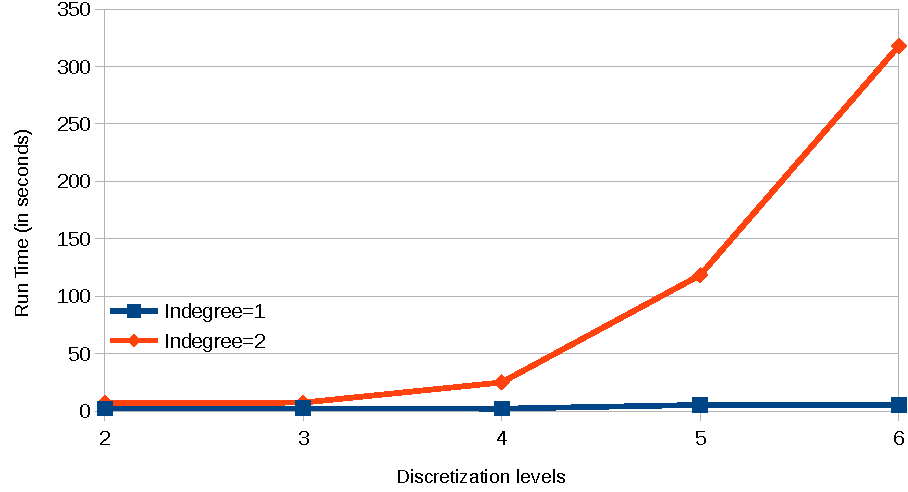
\includegraphics[width=0.33\linewidth]{images/net5}% TODO
	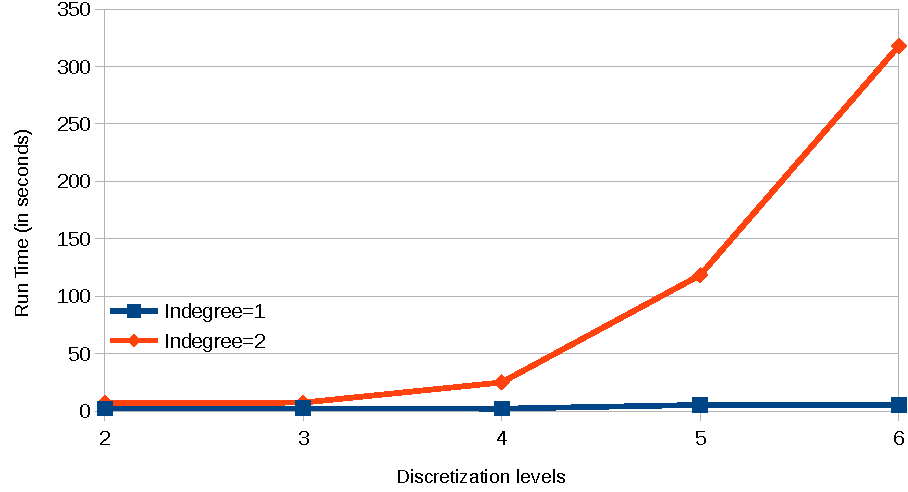
\includegraphics[width=0.33\linewidth]{images/net5}% TODO
	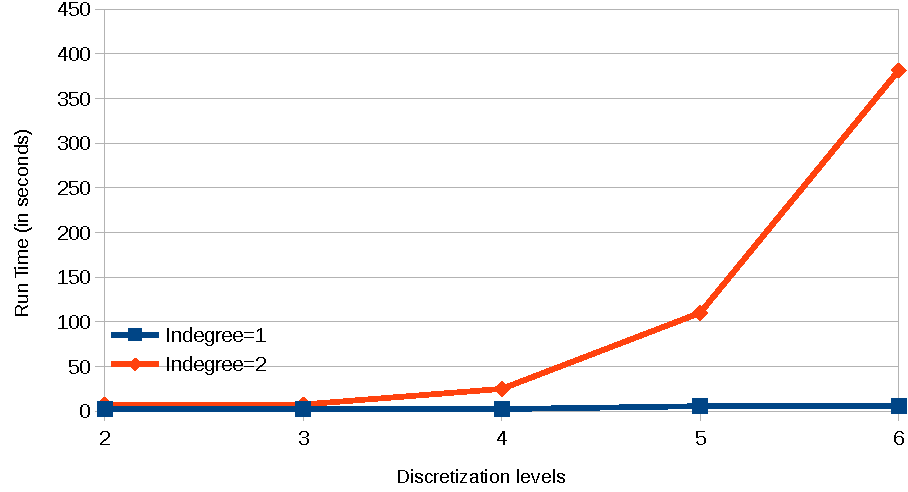
\includegraphics[width=0.33\linewidth]{images/net3}
	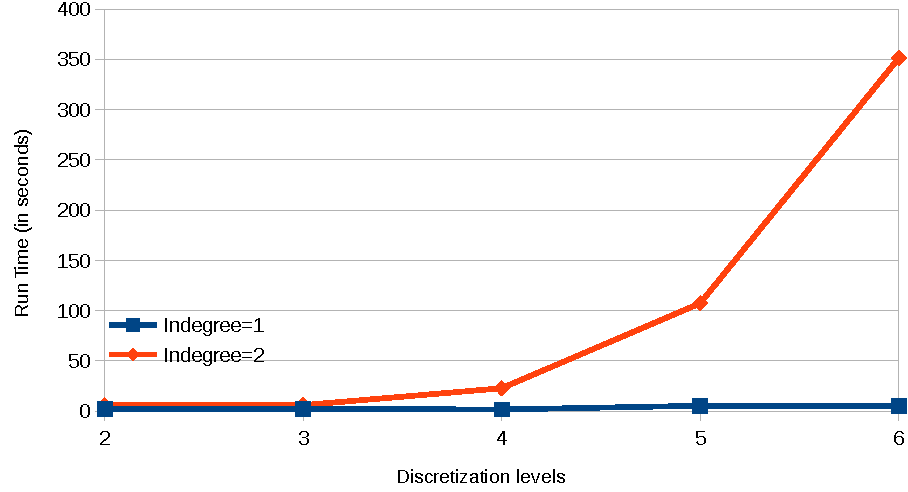
\includegraphics[width=0.33\linewidth]{images/net4}
	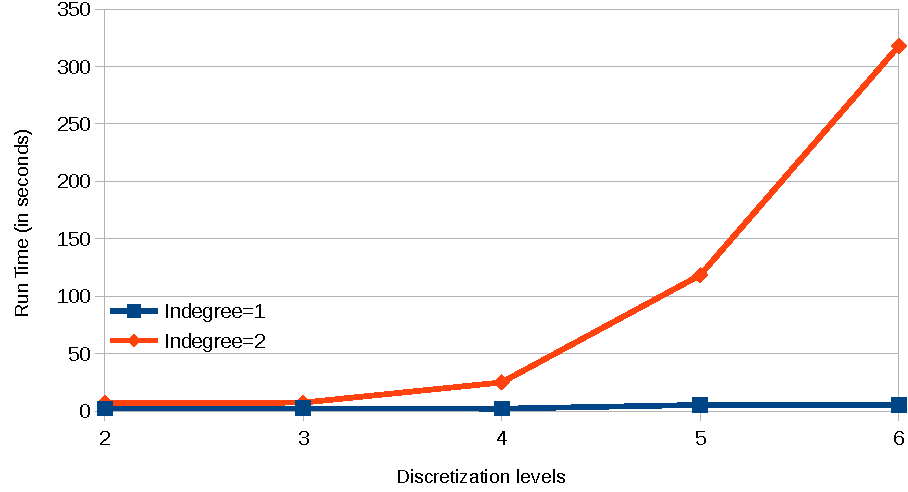
\includegraphics[width=0.33\linewidth]{images/net5}
	\label{fig:run_time}
	\caption{Evolution of run time on processing different network time series data from DREAM4 varying indregree of actions and discretization levels.}
	\end{figure}

	In the results optained from the experimentations of our algorithm on the time series data of the DREAM4 we can see the exponential influence on the run time of indegree of action considered as well as the level of discretization chosen.
	But it also show that in practice our approach can tackle big network, here 100 genes.

\textcolor{red}{COMMENT Tony: Faudrais testé en augmentant le nombre de time points si possible. Egalement avec un indegree de 3, 4 jusqu'a ce que ça soit trop long.}
